\documentclass[tikz,border=2pt]{standalone}
\usepackage{amsmath,amssymb}
\usepackage{tikz}
\usetikzlibrary{decorations.pathreplacing}

\begin{document}
% Per-unit money ladder for newspapers: price p = 5, cost c = 3.50, salvage s = 1.50.
% Underage b = p - c = 1.50 (margin missed on an unserved unit), overage h = c - s = 2
% (net loss on an unsold unit).
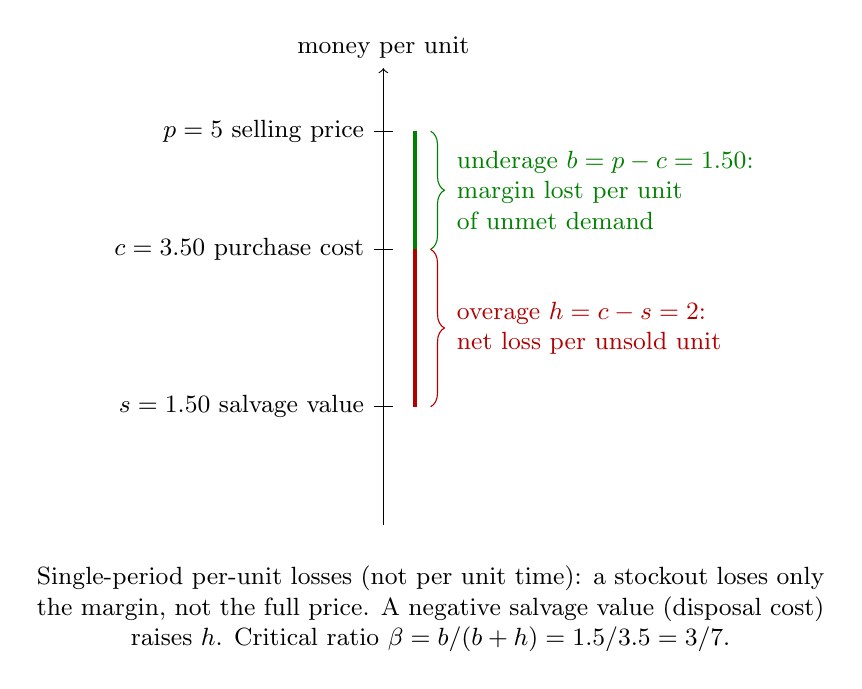
\begin{tikzpicture}[every node/.style={font=\small}, y=1.0cm]
	\draw[->] (0,0) -- (0,5.8) node[above] {money per unit};
	\foreach \v/\l in {5/{$p=5$ selling price}, 3.5/{$c=3.50$ purchase cost}, 1.5/{$s=1.50$ salvage value}} {\draw (0.12,\v) -- (-0.12,\v) node[left] {\l};}
	\draw[green!50!black, very thick] (0.4,3.5) -- (0.4,5);
	\draw[decoration={brace, amplitude=5pt}, decorate, green!50!black] (0.6,5) -- (0.6,3.5) node[midway, right=6pt, align=left] {underage $b=p-c=1.50$:\\ margin lost per unit\\ of unmet demand};
	\draw[red!70!black, very thick] (0.4,1.5) -- (0.4,3.5);
	\draw[decoration={brace, amplitude=5pt}, decorate, red!70!black] (0.6,3.5) -- (0.6,1.5) node[midway, right=6pt, align=left] {overage $h=c-s=2$:\\ net loss per unsold unit};
	\node[anchor=north, align=flush center, text width=10cm] at (0.6,-0.4) {Single-period per-unit losses (not per unit time): a stockout loses only the margin, not the full price. A negative salvage value (disposal cost) raises $h$. Critical ratio $\beta=b/(b+h)=1.5/3.5=3/7$.};
\end{tikzpicture}
\end{document}
